% ---
% Reemplaza líneas 986-1035 de Docs/Technical_Report.tex
% Decisiones: N/A (sin cambio)
% ---

\subsection{Fundamentos de computación cuántica}

El presente bloque introduce los conceptos y formalismos matemáticos de la computación cuántica que sustentan la implementación del circuito variacional desarrollado en este trabajo. La referencia estándar para esta sección es Nielsen y Chuang \cite{nielsen2010quantum}.

% -----------------------------------------------------------
\subsubsection{El qubit como unidad de información cuántica}
% -----------------------------------------------------------

La unidad fundamental de información en la computación cuántica es el \textit{qubit} (quantum bit). A diferencia de un bit clásico, que solo puede tomar los valores 0 o 1, un qubit puede encontrarse en una \textit{superposición} de ambos estados simultáneamente. Formalmente, el estado de un qubit se representa como un vector unitario en un espacio de Hilbert bidimensional $\mathcal{H} = \mathbb{C}^2$:

\begin{equation}
    |\psi\rangle = \alpha|0\rangle + \beta|1\rangle, 
    \quad \alpha, \beta \in \mathbb{C}, 
    \quad |\alpha|^2 + |\beta|^2 = 1
    \label{eq:qubit}
\end{equation}

\noindent donde $|0\rangle$ y $|1\rangle$ son los vectores de la base computacional estándar, análogos a los estados 0 y 1 clásicos:

\begin{equation}
    |0\rangle = \begin{pmatrix} 1 \\ 0 \end{pmatrix}, \qquad
    |1\rangle = \begin{pmatrix} 0 \\ 1 \end{pmatrix}
    \label{eq:basis}
\end{equation}

\noindent Los coeficientes $\alpha$ y $\beta$ son \textit{amplitudes de probabilidad}: al medir el qubit, se obtiene el estado $|0\rangle$ con probabilidad $|\alpha|^2$ y el estado $|1\rangle$ con probabilidad $|\beta|^2$. La medición es irreversible y colapsa el estado a uno de los dos valores de la base.

La representación geométrica estándar de un qubit es la 
\textit{esfera de Bloch}, que parametriza el estado general de 
un qubit (salvo fase global) mediante dos ángulos reales:

\begin{equation}
    |\psi\rangle = \cos\!\left(\frac{\theta}{2}\right)|0\rangle 
    + e^{i\varphi}\sin\!\left(\frac{\theta}{2}\right)|1\rangle,
    \quad \theta \in [0, \pi],\; \varphi \in [0, 2\pi)
    \label{eq:bloch}
\end{equation}

\noindent donde $\theta$ determina la mezcla entre $|0\rangle$ y $|1\rangle$, y $\varphi$ es la fase relativa entre ambos. Esta parametrización es fundamental para entender las compuertas de rotación que conforman los circuitos variacionales del presente trabajo \cite{nielsen2010quantum} (figura~\ref{fig:bloch}).

\begin{figure}[t]
    \centering
    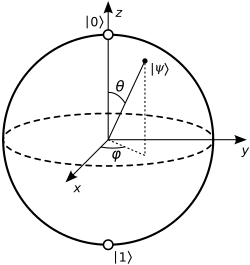
\includegraphics[width=0.3\textwidth]{Figures/Figura_3_1_1.png}
    \caption{Esfera de Bloch: representación geométrica de un qubit. 
    El estado $|\psi\rangle$ se representa como un punto en la 
    superficie de la esfera, determinado por los ángulos $\theta$ y 
    $\varphi$.}
    \label{fig:bloch}
\end{figure}
